
\subsection{Flavour-Tag Performance}
\label{sec:perf:hlr:lcfi}
The efficient identification of heavy flavour jets in hadronic events is an indispensable ingredient to many important physics analyses, such as
the $\PH\rightarrow\Pqc\APqc$ and $\PH\rightarrow\Pqb\APqb$ branching ratio  measurements.
The flavour tagging performance is studied using simulated and fully reconstructed samples
of dedicated $\Pep \Pem \rightarrow 6~\Pquark$ events at $\sqrt{s}=\unit{500}{\GeV}$, where all quarks are chosen to have the same flavour.
The samples are divided into two sub-samples, where one is used for training the BDT and the other is used
as a test sample. The resulting performance is shown in Fig.~\ref{fig:HLR-flavtag} for the large and small ILD detector model.
In (a) the background rate as a function of the c-tagging efficiency for b-quark and light flavour quark jets is plotted and (b) shows the
 background rate for c-quark and light flavour quark jets as a function of the b-tagging efficiency.
%
\begin{figure}[htbp]
\begin{subfigure}{0.49\hsize}
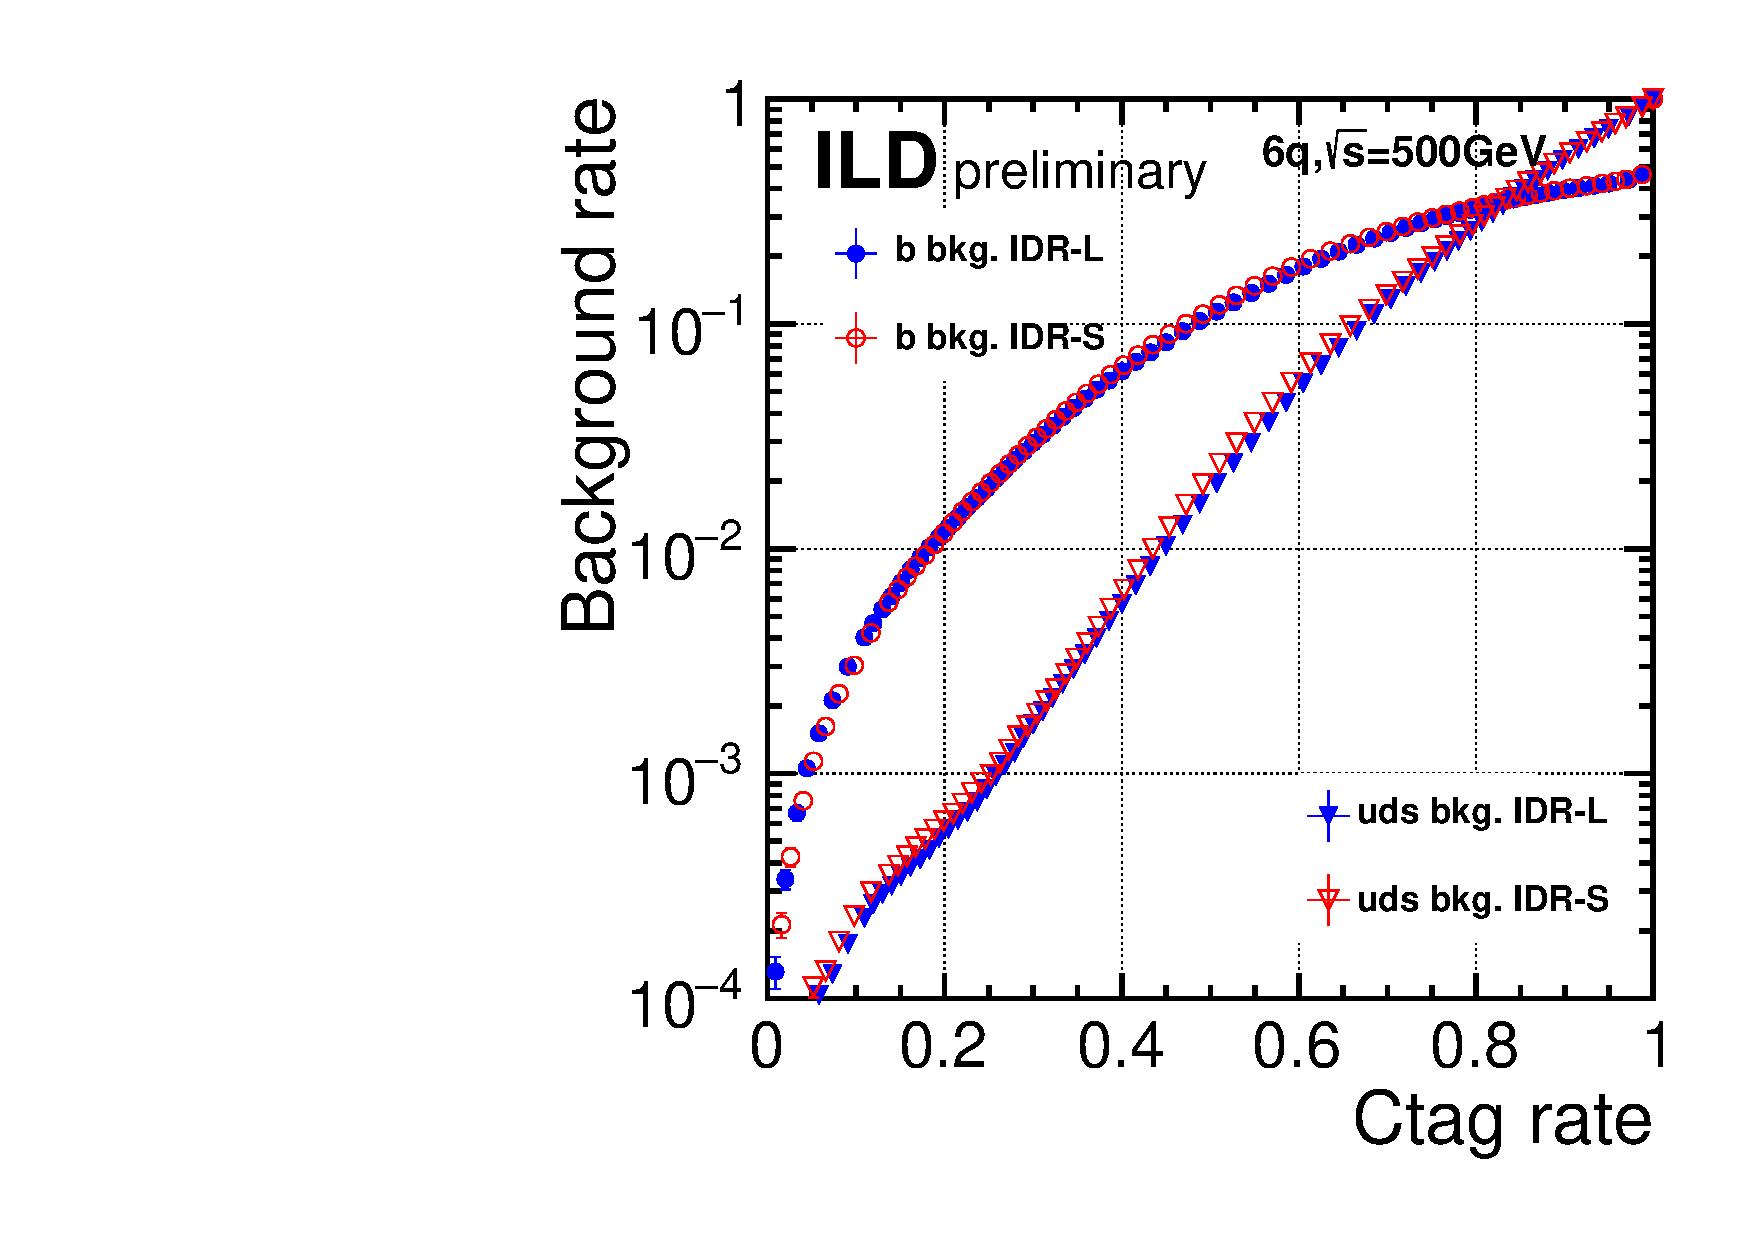
\includegraphics[width=\textwidth]{Performance/fig/ctag_performance.pdf}
 \caption{ \label{fig:HLR-ctag_perf}}
 \end{subfigure}
\begin{subfigure}{0.49\hsize}
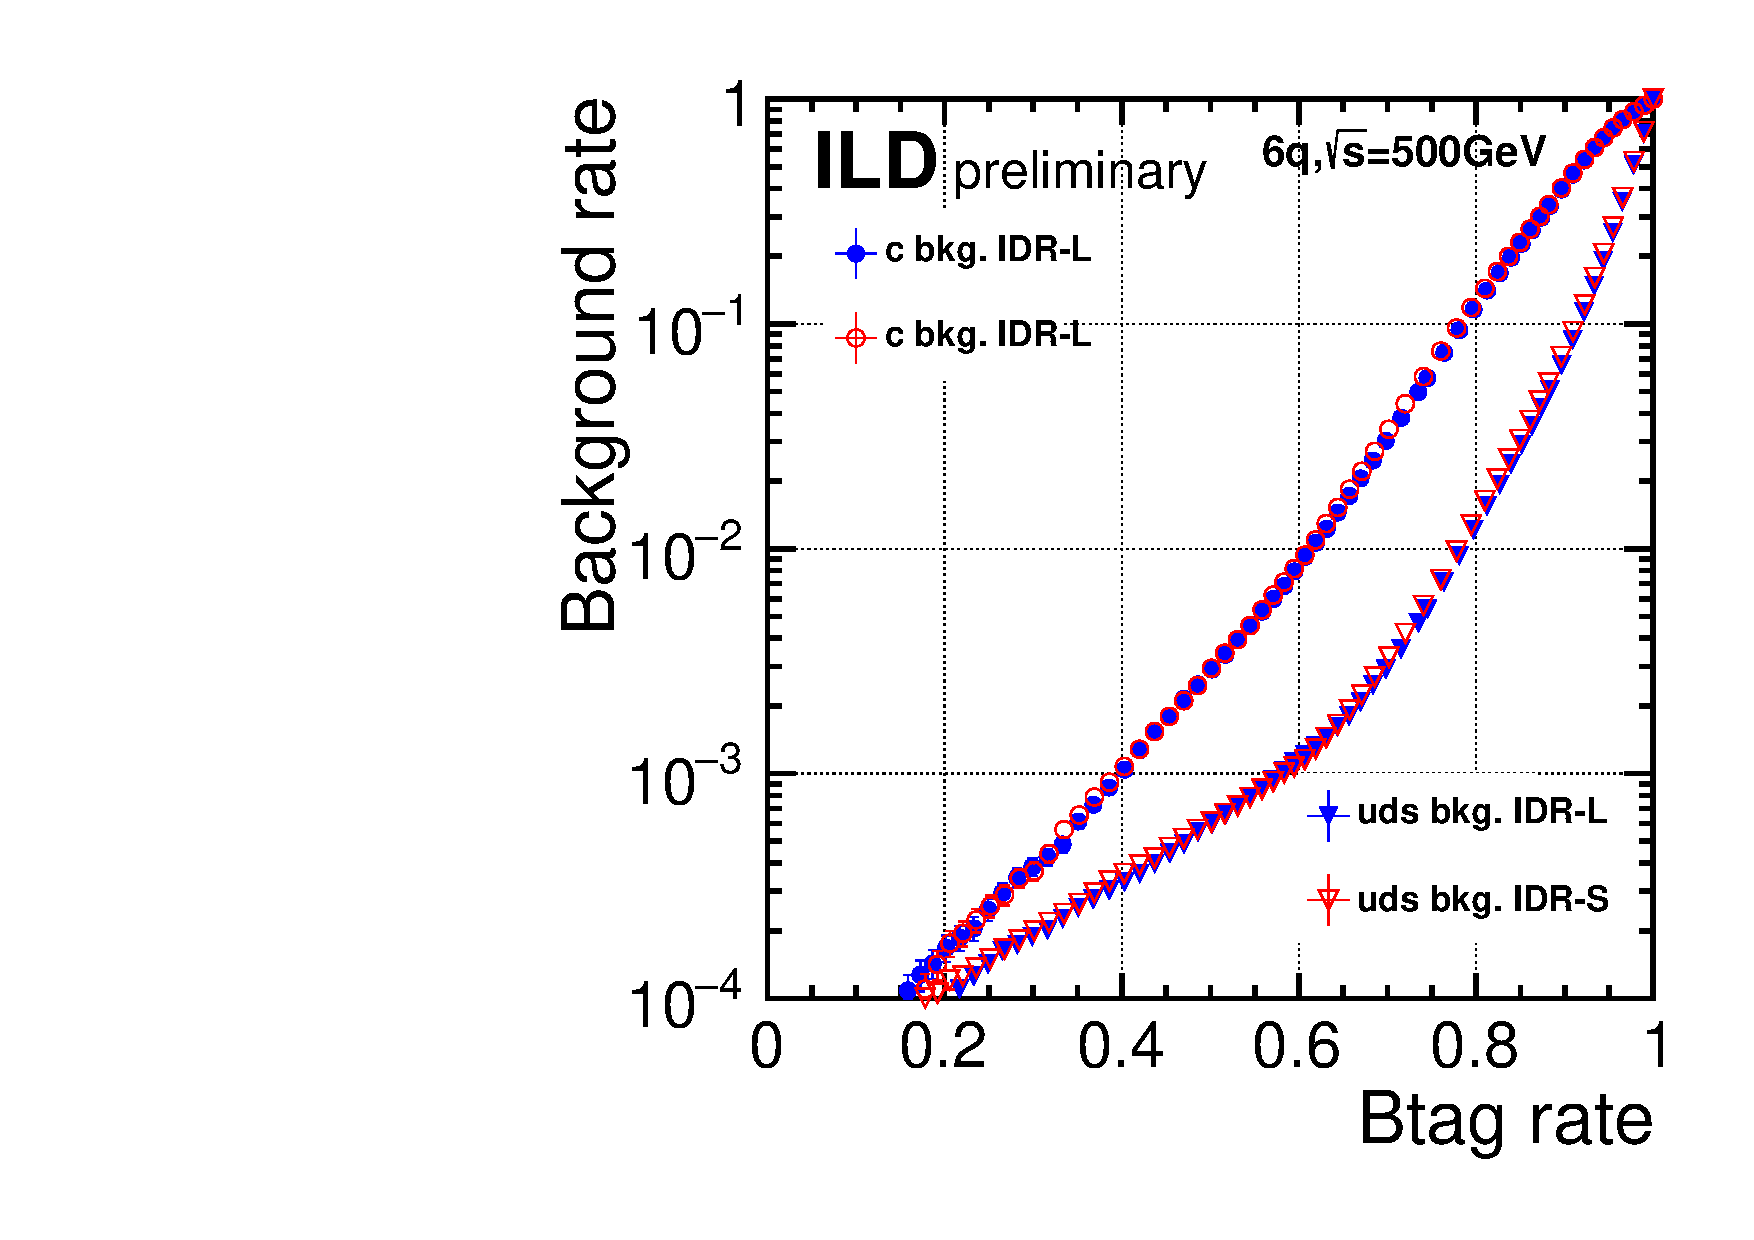
\includegraphics[width=\textwidth]{Performance/fig/btag_performance.pdf}
 \caption{  \label{fig:HLR-btag_perf}}
 \end{subfigure}
\caption{Flavour tag performance for the large and small ILD detector models. (a) background rate as a function of the c-tagging efficiency
  for b-quark and light flavour quark jets. (b) background rate as a function of the b-tagging efficiency for c-quark and light flavour quark jets. }
\label{fig:HLR-flavtag}
\end{figure}
%
As expected from the impact parameter and vertex resolutions there are no significant differences observed between the large and small ILD variants
for the flavour tagging performance.
The flavour tagging performance has been seen to vary with the jet energy and jet multiplicity~\cite{Suehara:2015ura}.
The ideal performance in a physics study can be achieved by retraining the BDTs for the corresponding signal event topology.
In practice, several sets of training weights are centrally produced, which are compared and chosen for the best performance.

%\subsection{neutral - \Ppizero}
\subsection{Hadronically decaying $\tau$ ID}
\label{sec:perf:hlr:tau}

The correct identification of $\tau$ lepton decay modes is of particular importance in the extraction of observables sensitive to the $\tau$ lepton spin direction: examples are measurements of the $\tau$ polarisation and Higgs CP based on spin correlations in $H \to \tau \tau$ decays.
Hadronic $\tau$ decays are typically offer the most sensitivity to the spin, due the presence of a single neutrino. 
The identification of these hadronic decay modes can be factorised into the charged and neutral components. 
The charged part is typically rather straight-forward in the TPC of ILD, so we concentrate efforts on understanding the identification of the neutral part, which consists largely of photons from neutral pion (and to a lesser extent other neutral meson) decays. 
In the decays of highly boosted taus, these photons are typically rather close to both a charged particle and one or more additional photons produced in the same $\tau$ decay. 
The separation between these photons in the calorimeter depends on its inner radius, while the distance to charged particles additionally depends on the magnetic field strength. 
We can therefore expect some differences in performance for the large and small ILD detector models.

The performance of $\tau$ decay mode identification was studied in $\tau$-pair production events at a centre-of-mass energy of $500$\,GeV. 
These very highly boosted $\tau$ decays are the most challenging to reconstruct due to the small distance between particles in the highly collimated $\tau$ decay jets.
The standard ILD reconstruction algorithms were applied to these events.

In each event, two high momentum, back-to-back, charged PFOs were identified as $\tau$ jet "seeds". Figure~\ref{fig:HLR-tauID} shows the number of photon PFOs identified in a cone around these $\tau$ seed tracks, in the case when the $\tau$ lepton decayed to $\pi^\pm \pi^0 \nu$.
In these events, exactly two photons are expected in the vast majority of cases. 
The distribution shows that it is challenging to reconstruct both photons: in around half of the cases only a single photon cluster was reconstructed, which is due to the merging of the two photons into a single reconstructed particle. 
A difference is seen between the two detector models, with the large version somewhat more often correctly resolving the two photons, which can be understood as being due to the larger ECAL radius increasing the distance between the photons' electromagnetic showers.


\begin{figure}[htbp]
\begin{subfigure}{0.49\hsize} 
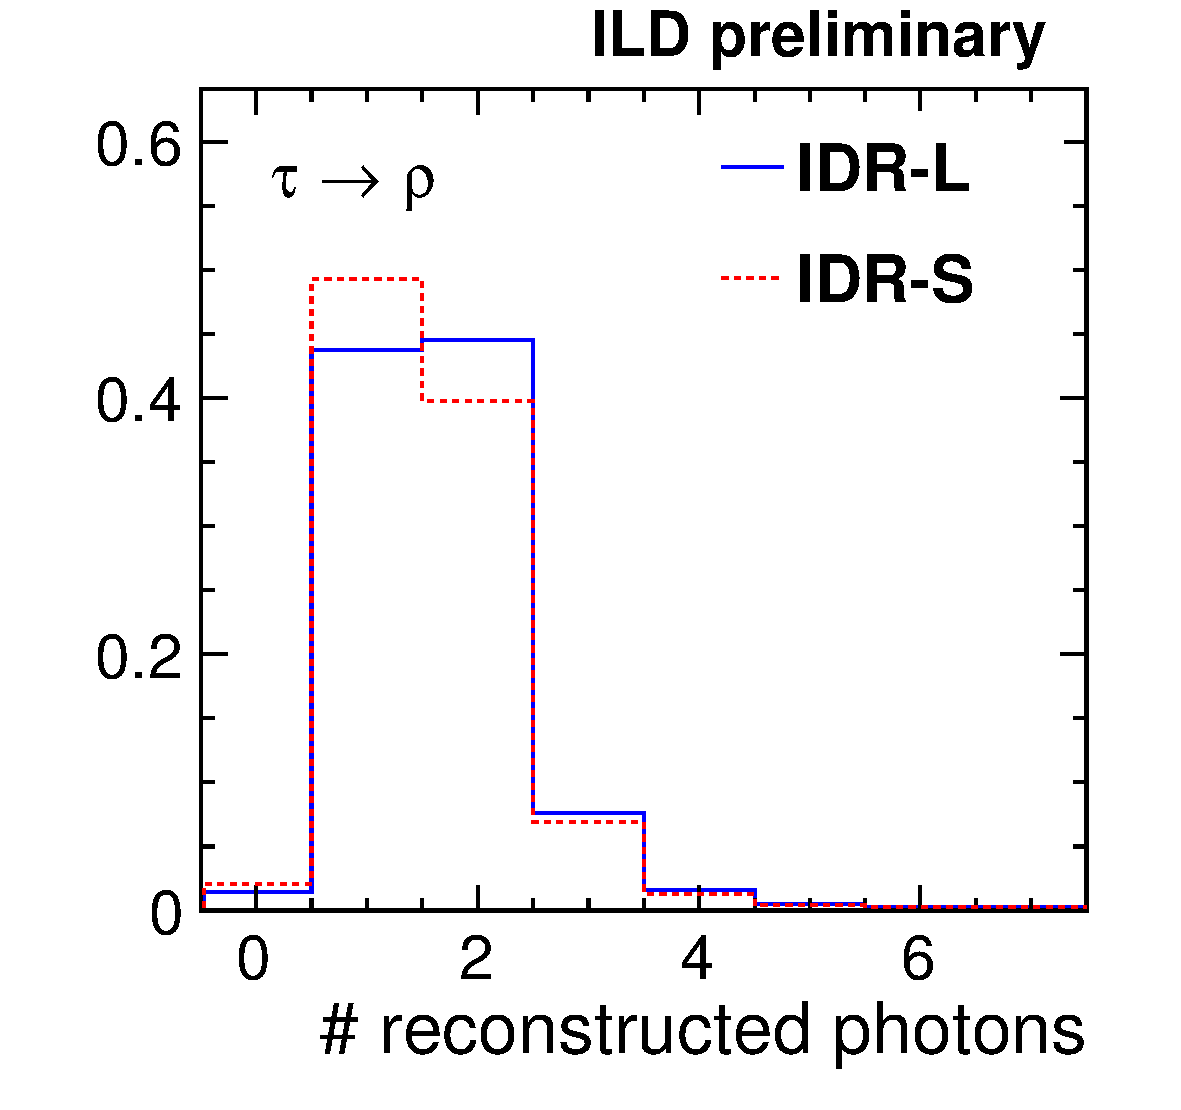
\includegraphics[width=\textwidth]{Performance/fig/tauID_ngammapfo.pdf}
 \caption{ \label{fig:HLR-tauID:ngamma}}
 \end{subfigure}
\begin{subfigure}{0.49\hsize} 
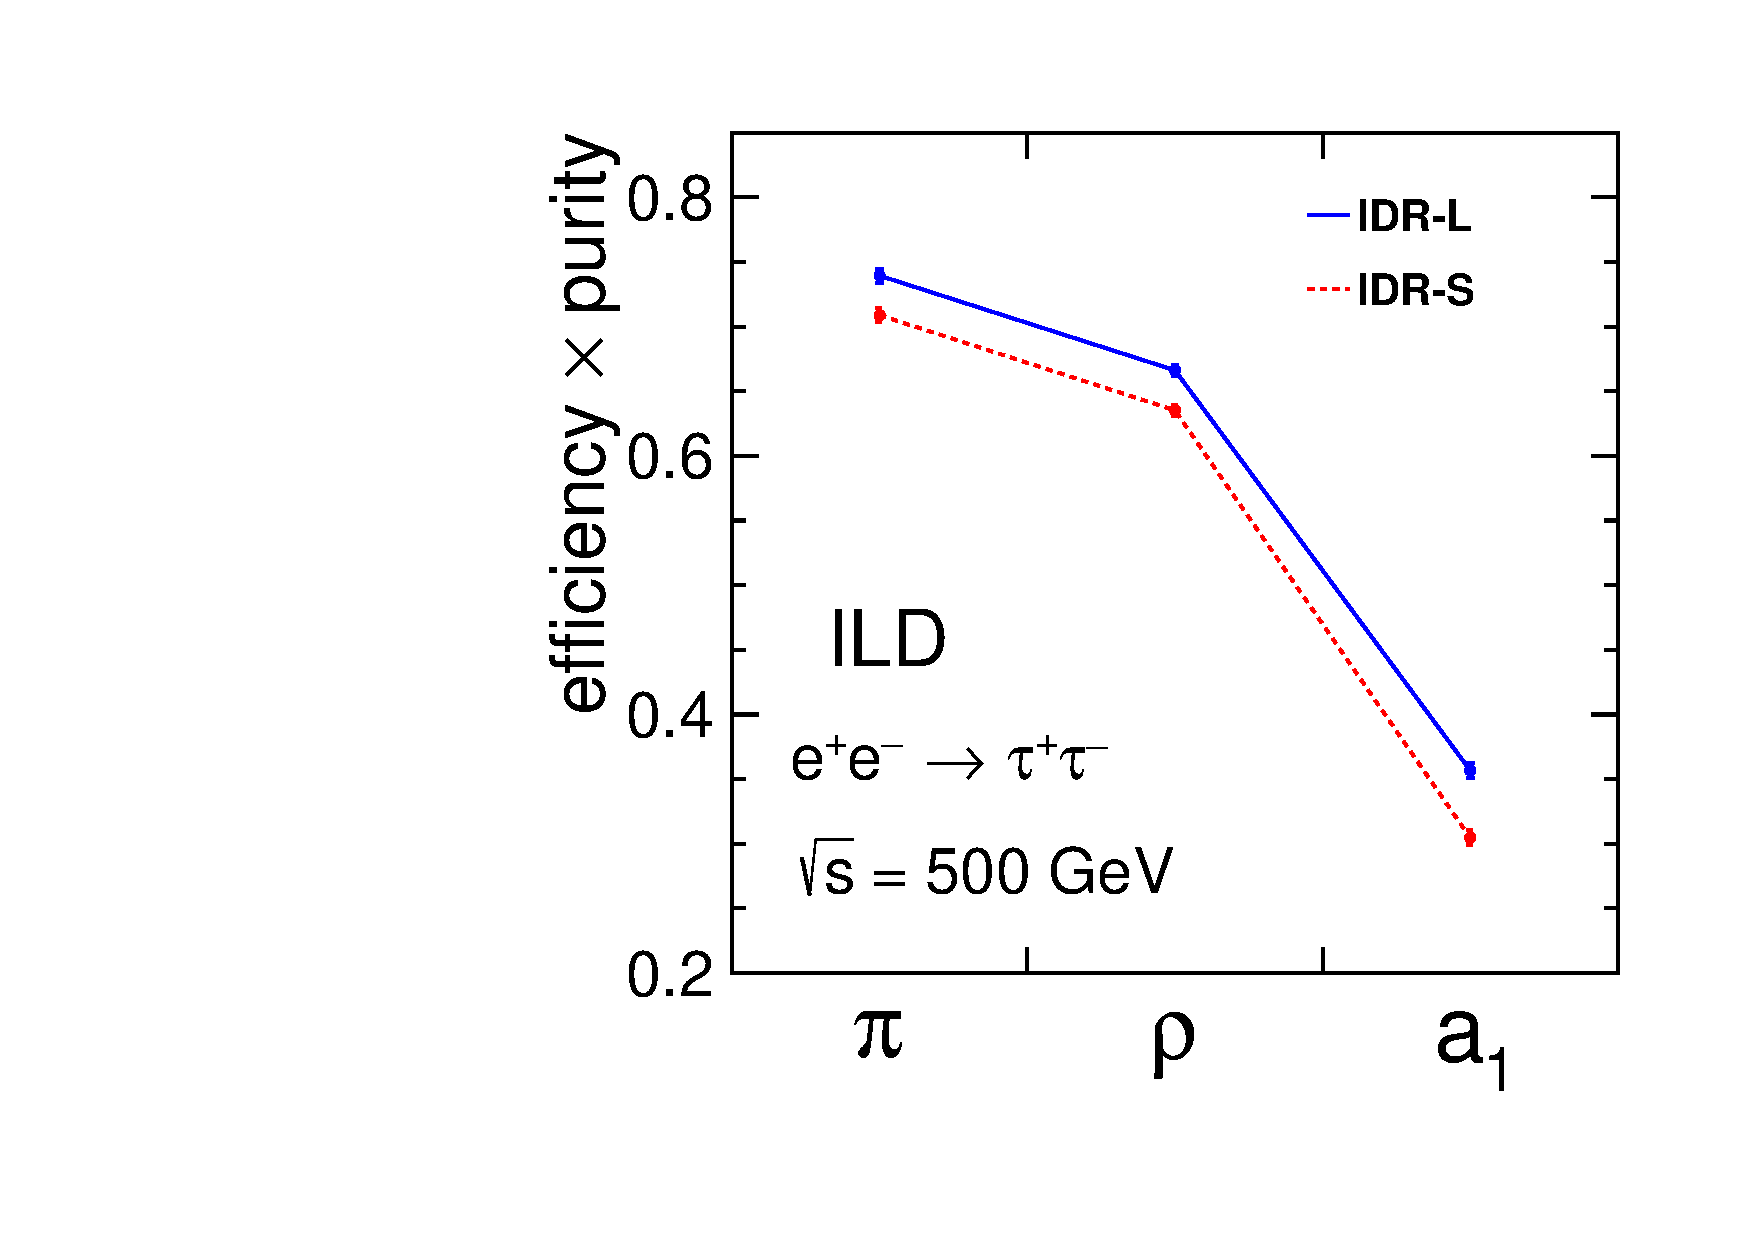
\includegraphics[width=\textwidth]{Performance/fig/tauID_effPur.pdf}
 \caption{  \label{fig:HLR-tauID:effpur}}
 \end{subfigure}
\caption{Hadronic decay mode identification for isolated $\tau$-leptons with momenta near $250$\,GeV.
(a) The number of reconstructed photon PFOs in  $\tau \to \rho \nu \to \pi^\pm \pi^0 \nu$.
(b) The performance of a simple $\tau$ decay mode identification algorithm.
}
\label{fig:HLR-tauID}
\end{figure}


A simple cut-based approach to the identification of single-prong hadronic $\tau$ decays was developed, based on the number of reconstructed photon PFOs, and the invariant mass of this set of photon PFOs both alone and together with the charged PFO around which the $\tau$ candidate jet was built.
The ability of this algorithm to distinguish $\tau \rightarrow \pi^\pm \nu$ ("$\pi$"), $\tau \rightarrow \pi^\pm \pi^0 \nu$ ("$\rho$"), and $\tau \rightarrow \pi^\pm \pi^0 \pi^0 \nu$ ("$\mathrm{a_1}$") decays is shown in Fig.~\ref{fig:HLR-tauID}. 
The product of selection efficiency and purity varies between around 30\% and 75\% among these three decay modes.
The large detector model performs slightly better, as expected thanks to the larger inner ECAL radius.

%\subsection{V0 / in flight decays vs radius}
\subsection{$J/\psi$ reconstruction}
With the excellent particle flow, particle identification and vertexing capabilities
of ILD discussed in the previous sections, there is a great potential to reconstruct
various exclusive decay chains of short-lived baryons and mesons. This is of special
interest in case the ILC will be operated at the $Z$ pole, but also at higher energies we expect further improvements to flavour tagging and jet energy resolution
once this potential is fully exploited in reconstruction and analyses. This is an area where new algorithmic developments could still lead to a significant improvement
of the ILD performance.

At the current stage, we only provide a very simple example, namely the reconstruction of $J/\psi \to \mu^+\mu^-$ decays. Due to its extremely well-known mass (known to 3.6\,ppm~\cite{Tanabashi:2018oca}), the $J/\psi$ is an important standard candle, e.g.\ for calibration of the tracker momentum scale.

\begin{figure}[htbp]
\begin{center}
 \includegraphics[width=0.75\textwidth]{Performance/fig/Jpsi_InvMassS5_vs_L5.pdf}
\end{center}
\caption{$J/\psi \to \mu^+\mu^-$ candidates as reconstructed with IDR-L and IDR-S.}
\label{fig:hlr:jpsi}
\end{figure}

Figure~\ref{fig:hlr:jpsi} shows the invariant mass spectrum of reconstructed muon pairs in the $J/\psi$ region, comparing the large and small detector. All available
SM MC events from the optimisation production at $\sqrt{s}=500$\,GeV have been used and weighted to the full luminosity of $4$\,ab$^{-1}$ with the canonical sharing between the polarisation configurations. The combinatorial background has been determined from like-sign muon pairs and has been subtracted from the opposite-sign pairs, leading to the fluctuations around zero in the off-peak regions.
At $500$\,GeV, most $J/\psi$ candidates are produced in the forward direction, with $|\cos{\theta}|>0.8$ and at rather low transverse momenta, typically below $30$\,GeV.
Therefore, the small detector has a smaller acceptance than the large detector, with about $10$k vs $12$k recontructed $J/\psi$'s compared to about $20$k available at generator level. On the other hand, the better momentum resolution of the small detector in the forward region leads to a more narrow peak.
% \fix{
% \begin{itemize}
% \item $\Lambda^+_c \to pK^- \pi^+$
% \item $D^0$, $D^*$
% \item $J\psi \to \mu \mu$  / inclusive di-muon spectrum ?
% \end{itemize}
% }

% \subsection{Di-jet mass resolution between Cambridge and full physics}
% \begin{itemize}
% \item $Z$ mass in $ZZ \to \nu\nu qq$, flavour separated
% \item $W$ hadronic mass from $WW \to qq l\nu$
% \item from Jakob $\nu\nu qqqq$
% \item various levels of cheating with TrueJet
% \end{itemize}

